%-------------------------------------------------------------------------------------------------------
%-------------------------------------------------------------------------------------------------------
% Sec & Label

\section{Theoretical Analysis}
\label{sec:analysis}


%-------------------------------------------------------------------------------------------------------
%-------------------------------------------------------------------------------------------------------
% Intro

In this section we will explain the inner workings of the AC/DC converter created and perform a theoretical analysis of each component. For the analysis it was assumed that each component only affects the components that come after it and so does not interfere with the previous analysis.
The common Kirchoff laws and diode equations (simplified in some cases) were used to perform the analysis.

%-----------------------------------------------------------------------
%-----------------------------------------------------------------------
% 		     	    Transf - subsec
% ----------------------------------------------------------------------
% ----------------------------------------------------------------------

\subsection{Transformer}
\label{subsec:transf}

The transformer is the component that steps down the supplied voltage. This step is necessary to approximate the supplied 230V to the 12V required. Since it was assumed that the transformer was ideal, its response can me modeled as a simples change in amplitude, that is related with the number of windings by the following equation:
V_out=V_in/n

%-----------------------------------------------------------------------
%-----------------------------------------------------------------------
% 		     	    EnvDet - subsec
% ----------------------------------------------------------------------
% ----------------------------------------------------------------------

\subsection{Envelope Detector}
\label{subsec:envdet}

The envelope detector is comprised of two sub-components: The rectifier and a filter.
The chosen rectifier for our application was the Full-Wave Bridge Rectifier. The purpose of a rectifier is to turn the AC component of the supply to a DC current. To accomplish this objective the rectifier uses four diodes positioned in a way as to only allow the current to pass one way (shown in diagram).
This behavior was achieved in octave by performing the abs() function to the signal and subtracting 2 times the diode’s V_on voltage (simulating the two diodes the current has to pass through using the V_on model).
The filter is comprised of a series resistor and parallel capacitor. Its objective is to stabilize the signal and decrease the voltage ripples caused by the rectifier. This behavior was computed in matlab by comparing the signal voltage at each moment with the equivalent RC circuit voltage, the larger of the two was chosen to be the signal.

%-----------------------------------------------------------------------
%-----------------------------------------------------------------------
% 		     	    Optim - subsec
% ----------------------------------------------------------------------
% ----------------------------------------------------------------------

\subsection{Voltage Reg}
\label{subsec:voltreg}

This component has the objective of limiting the voltage to the desired value and at the same time, by using the non-linear behavior of a diode to decrease oscillations in the signal.
The component is comprised of 17 diodes in series to achieve the desired voltage.
Incremental analysis performed to find the final output signal.

%-----------------------------------------------------------------------
%-----------------------------------------------------------------------
% 		     	    Optim - subsec
% ----------------------------------------------------------------------
% ----------------------------------------------------------------------

\subsection{Optimization}
\label{subsec:optim}

As a consequence of not being given any values, the group had to optimize the values
for each component in order to obtain tha highest Merit possible. Thus, an Octave script
was written to give us the optimal values.


%-----------------------------------------------------------------------
%-----------------------------------------------------------------------
% 			     Results - subsec
% ----------------------------------------------------------------------
% ----------------------------------------------------------------------

\subsection{Theoretical Results}
\label{subsec:res_the}

\begin{figure}[ht]
	\centering
	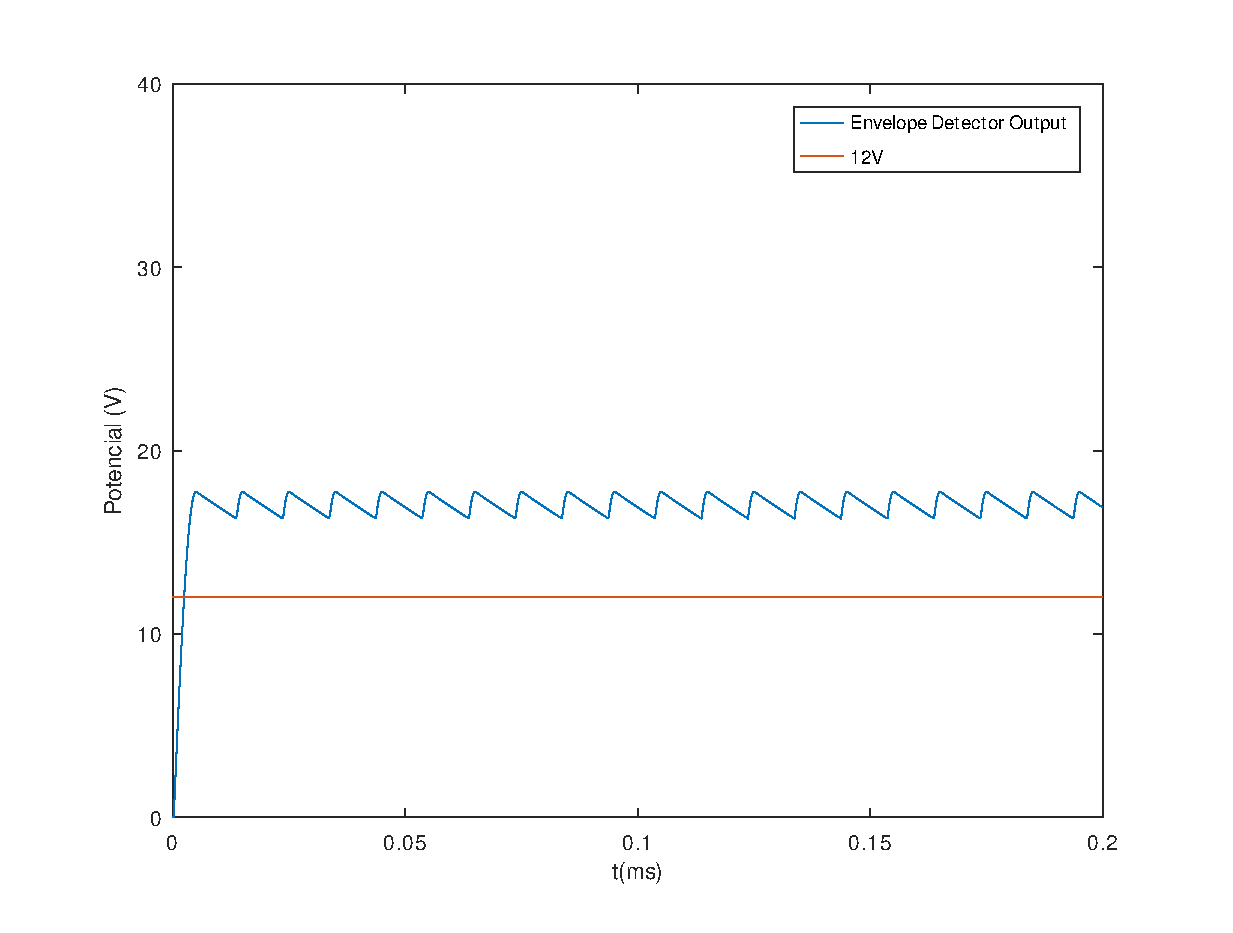
\includegraphics[width=1\linewidth]{envelope_detector.eps}
	\caption{Envelope Detector Circuit $v_{out}$}
\label{fig:EV_vout_a}
\end{figure}

\begin{figure}[ht]
	\centering
	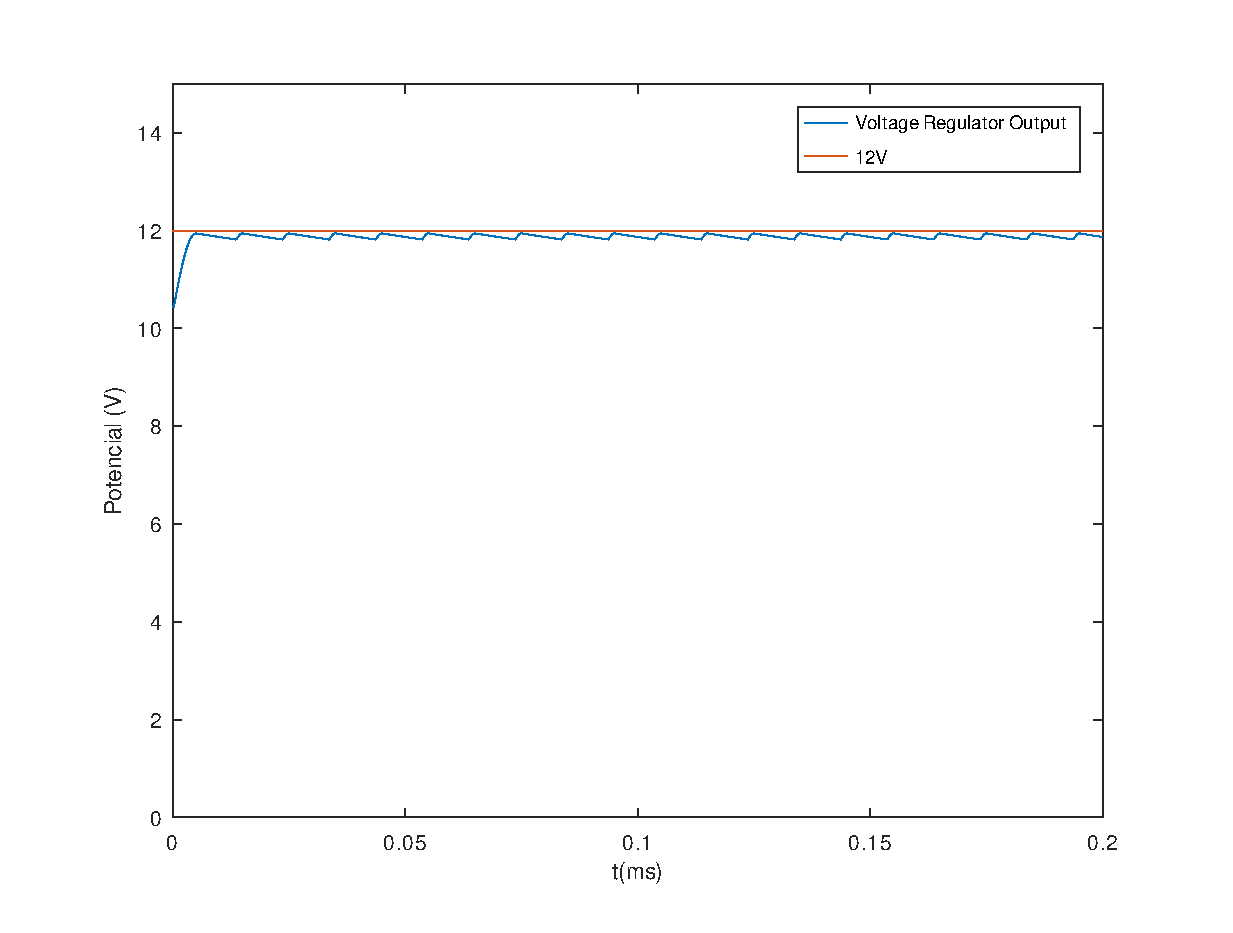
\includegraphics[width=1\linewidth]{voltage_regulator.eps}
	\caption{Voltage Regulator Circuit $v_{out}$}
\label{fig:VR_vout_a}
\end{figure}

